\chapter{Preliminary material: quantitative methods}
\label{chapter:introductory_material}

The work in this thesis builds upon the foundations built by decades
of research in the development of machine learning.  In this chapter,
I will describe enough of these foundations for the reader to
understand later chapters. Some of this work builds off of general
knowledge in the machine learning community; when the foundational
work is beyond the scope of this introduction, I will provide
references to well-known resources in the community.

In this chapter I will outline the basic methodology for
probabilistic modeling in datasets.  I begin by discussing a ``data
analysis pipeline'' so the reader will understand what is meant by
phrases like ``the data'', ``fit the model'', and ``heldout
log-likelihood'', and where it falls in the overall research pipeline.
I then provide basic definitions from the field of probabilistic
modeling and illustrate these ideas with models that will be used as
building blocks in later chapters.

\section{Standards and naming conventions}
I begin by outlining naming and variable conventions in this work.
Random variables and their instantiations are given by roman or greek
characters; the role of a variable will typically be evident from its
context.  Multivariate random variables such as vectors are given by
boldface, and collections of random variables are given by uppercase
Roman characters.

The reader may find \mytab{notation} a helpful resource in the
subsequent chapters.  This table summarizes many of the variables
described in this work.

When we refer to a variable, we will sometimes subscript it with
multiple indices.  For example, in the next chapter, we will refer to
the probability $\beta_{t,k,n}$ of word $n$ in topic $k$ at time
$t$. We sometimes refer to only a subset of these indices. In such
cases, we are referring to the appropriately-shaped variable:
$\beta_{t,k,n}$ is a scalar; $\beta_{t,k}$ and $\beta_{k,n}$ are
vectors; $\beta_t$ and $\beta_k$ are matrices; and
$\beta$ is a three-dimensional tensor.  In the interest of brevity and
clarity, the shape of such variables will be understood from context.

\label{sec:pipeline}

\section{Latent-variable models, prediction, and exploration}

\subsection{Data analysis pipepline}
\label{sec:data_analysis_pipeline}
We will develop the ideas outlined in the last chapter by using the
``data analysis pipeline'' illustrated in
\myfig{data_analysis_pipeline}.\footnote{This pipelne is very much
  inspired by discussions with David Blei.}  This pipeline, which
is driven by a specific question about a set of data, serves as a
recipe for answering questions about these data.  It will also help to
make the contributions of this thesis more explicit.

The pipeline has several important steps.

\begin{enumerate}
\item \textbf{Questions.} One of the first, most critical steps is
  defining the question at hand.  In our case, the questions include
  ``Which articles are of interest to the field of historiography?''
  and ``How do lawmakers feel about specific issues?''. Notice that
  these questions may have multiple answers.

\item \textbf{Data.} At the same time we are formulating questions, we
  must also understand which set of data will allow us to address the
  question at hand.  Of course, the questions we ask will be informed
  by the data available to us, and vice-versa.

\item \textbf{Modeling assumptions.} Once we have established a set of
  questions and available data, we define a set of assumptions that
  will allow us to capture statistics of interest.  When we analyze
  lawmakers' issue preferences, for example, we will make assumptions
  about how lawmakers feel about issues and how they interact with
  bills.  We will encode these assumptions by specifying them with
  random variables.

  This step arguably allows the practitioner wide latitude in defining
  variables of interest.  In following chapters, we will spend a lot
  of time discussing modeling assumptions, and they compose one of the
  biggest contributions of this work.

  Just as the \textbf{Data} step is limited by the questions we are
  asking, the, our decisions in the \textbf{Model assumptions} step
  are informed by limitations in the tools available for performing
  inference and the ease of subsequent data analysis.

  \item \textbf{Model implementation.} In this stage, the model is
  defined, and the practitioner must encode these modeling assumptions
  into an algorithm and run that algorithm.  We will variously refer
  to this stage of the process as \emph{fitting a model},
  \emph{performing inference}, and \emph{fitting the posterior}.  This
  steps also represents a significant contribution of our work, in
  chapters 3-6 and Appendix A.

  \item \textbf{Model evaluation.} The goals of this stage are to
    evaluate performance of the model and to criticize the model.
    The criticism may warrant model revision, in which case the
    modeling assumptions are adjusted, the model is refit, and the
    model is re-evaluated.

    Model criticism can take many forms, including prior and posterior
    checks \citep{box:1980,gelman:1996} and measures of the model's
    ability to predict held-out observations. We will primarily focus
    on evaluating models based on external measures, although we will
    also include internal metrics such as the predictive
    distribution. When appropriate, we will also incorporate standard
    metrics for topic model evaluation \citep{wallach:2009}.
  
  \item \textbf{Conclusions.} Finally, the practitioner may draw
    conclusions from the model.  In our case, this leads to two
    applications: \emph{exploration} and \emph{prediction}.  Models
    built for exploration can be used to answer potential \emph{future}
    questions about the data with the guidance of a human (``Which
    lawmakers are most right-wing on foreign policy?  How does Ron
    Paul feel about Taxation?'').  Models
    build for prediction can be used to draw specific inferences about
    unseen or future information (``How will Ron Paul vote on the
    pending taxation bill?'').

    It is worth pointing out the other types of conclusions that one
    may draw in this stage, but which we will not discuss. Some
    researchers may define their models with very specific questions
    in mind (``Has Ronald Paul sided more with Democrats than
    Republicans on wartime spending since the 2003 Iraq invasion?'').
    Others may draw causal conclusions (``The Iraq war caused Ronald
    Paul to favor wartime spending less''). These are interesting
    questions with fascinating solutions, but they require domain
    knowledge which we will not assume.

    Finally, it is worth noting that exploratory analysis is a large
    field of study.  We will focus on modeling assumptions and
    immediate corollaries that we can draw from the data.  For
    completeness, we note that many researchers create tools to
    display information meaningfully to -- and elicit interaction with
    -- users.  Well-known sources for display of this information
    include \cite{tufte:2001} and \cite{wilkinson:2005}, while
    visualization tools for models like those in this work have been
    developed by \cite{chaney:2012}.

\end{enumerate}

\begin{figure}
  \center 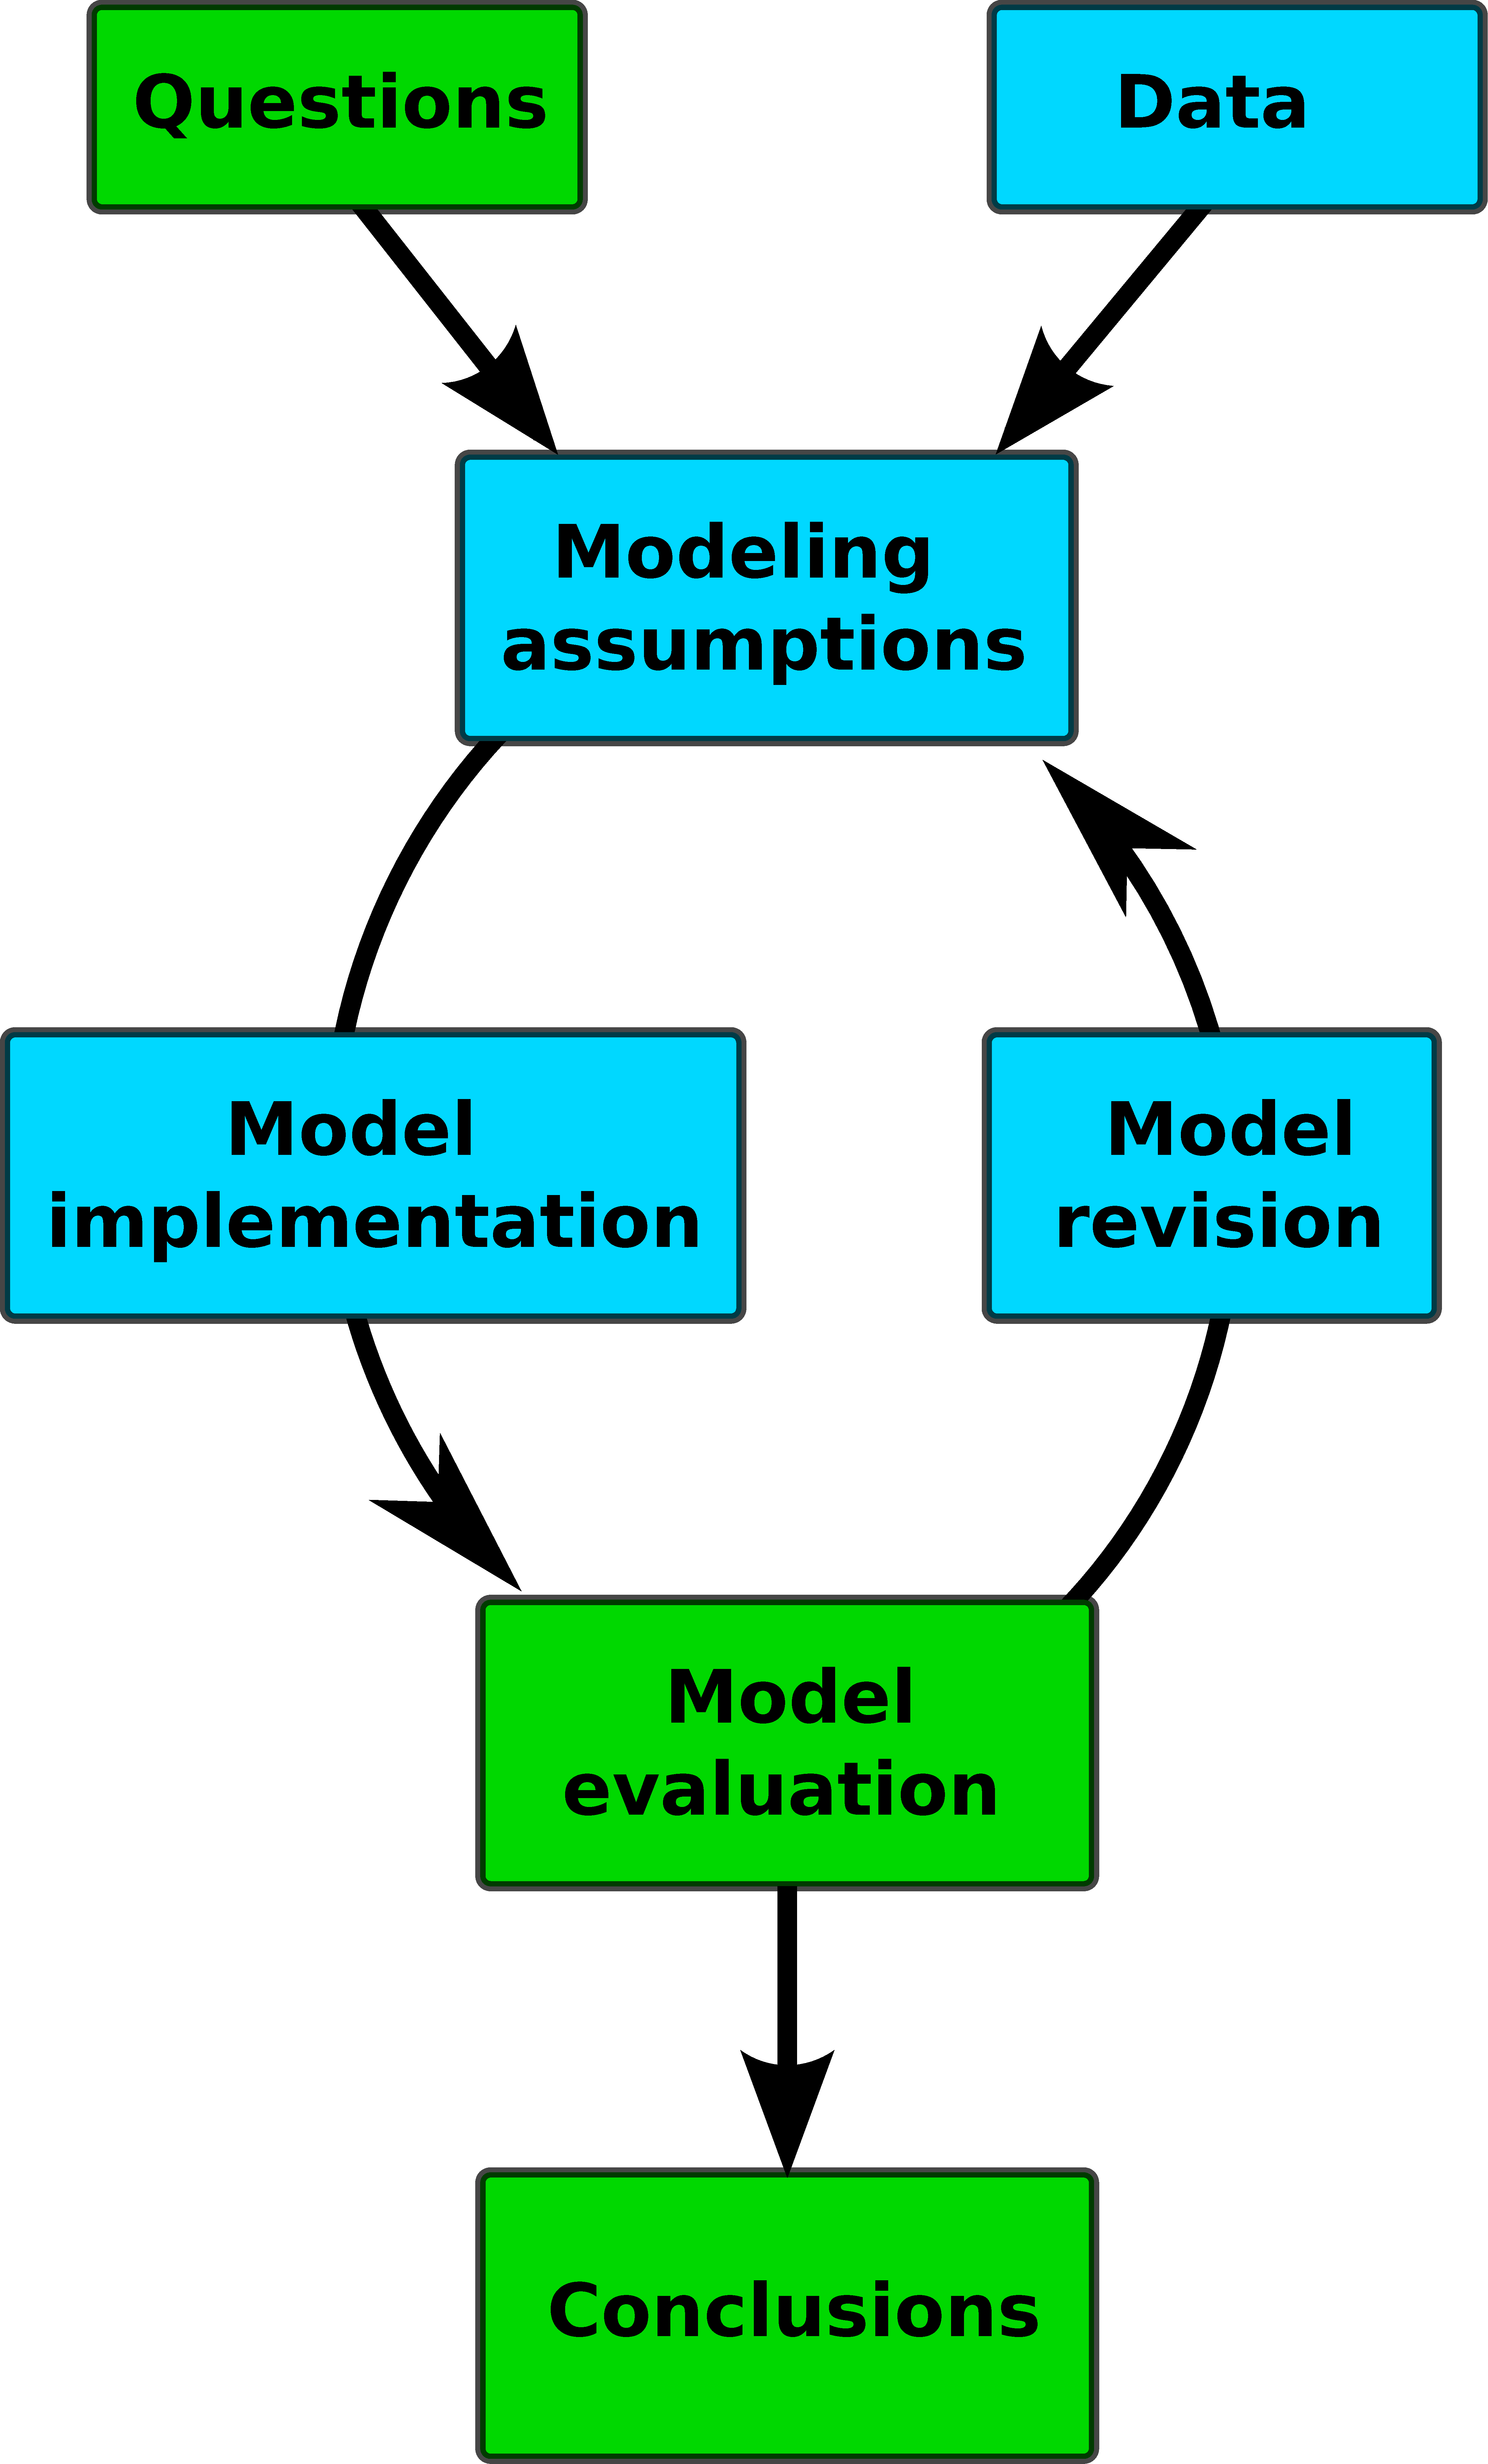
\includegraphics[width=0.4\textwidth]{chapter_introductory_material/figs/model_pipeline.pdf}
  \caption{A data analysis pipeline.  In this work, we make
    contributions in the areas of \textbf{Modeling assumptions},
    \textbf{Model implementation}, and \textbf{Model revision}.  We
    will focus on applications which use text data.}
  \label{fig:data_analysis_pipeline}
\end{figure}

As alluded to above, this work will focus on modeling assumptions and
model implementation.  To encode our assumptions, we will use latent
variable models because they have several clear benefits.

\subsection{Latent-variable models}

To formalize what we mean by \emph{Modeling assumptions}, we will
assume that observed data can be described by a probability
distribution.  By making this assumption, we will gain several
benefits, which we outline at the end of this section.  First, we
formalize a \emph{latent variable model}.  A latent variable model can
be fully specified with
\begin{itemize}
  \item A set of latent random variables $X_1, \ldots, X_{M_1}$ ($X_{1:M_x}$ for shorthand);
  \item A set of observed random variables $Y_1, \ldots, Y_{M_2}$ ($Y_{1:M_y}$ for shorthand);
  \item A joint probability distribution $p(X_{1:M_x}, Y_{1:M_y})$.
\end{itemize}
While some practitioners may index the distribution $p$ with some
index set $\{ \theta \}$ with the goal of learning that index $\hat
\theta$ which makes the data most likely, we will usually focus on a
single distribution and use a Bayesian treatment of the problem.  As
$p$ is a probability distribution, it satisfies
\begin{align*}
  \int_{x_{1:M_x}, y_{1:M_y}} p(X_{1:M_x}, Y_{1:M_y}) d x_{1:M_x}, d
  y_{1:M_y} = 1.
\end{align*}
  
For $p$ to be useful, we typically will make distributional
assumptions about it.  We often describe assumptions about
factorization using a \emph{directed graphical model} (sometimes
called a Bayesian network) \citep{pearl:1985}.\footnote{Undirected
  graphical models are also useful.  Here we focus on undirected
  graphical models.}  A graphical model is a directed, acyclic graph
$G = (V, E)$ in which vertices $V=1, \ldots, M = M_x + M_y$ index
random variables and a \emph{lack} of edges between random variables
connotes conditional independence.

We state this more precisely be defining the ``parents'' function
$\pi_G : \{ 1, \ldots, M \} \rightarrow 2^{\{ 1, \ldots, M \}}$, which
takes the random variable index $m$ to its parents $\{ i : i \neq m
\mbox{ and } (Z_i, Z_m) \in E \}$.  By definition, a probability
distribution described by a graphical model $G$ can be factorized as
\begin{align}
  p(Z_1, \ldots, Z_M) = \prod_{i=1, \ldots, M} p_\theta(Z_i | \pi_G(Z_i) ).
\end{align}
Note that there is a many-to-many relationship between graphical
models and probability distributions. Each graphical model may
describe many different distributions (but all such distributions must
be factorizable based on this graphical model).  Likewise, each
probability distribution can be described by multiple graphical
models (but each distribution must be factorizable based on all of its
corresponding graphical models). The language of graphical
models makes it possible to succinctly describe many joint probability
distributions, and it makes model implementation and inference with
these models much easier to discuss formally.

Conventionally, a graphical model $G$ is often drawn as a
block-and-arrow diagram, where we write out the graph with each random
variable (vertex) drawn as a circle and each edge edge drawn as an
arrow.  An additional convention in these diagrams is that boxes, or
\emph{plates}, represent replication (with the number of replications
shown in a corner of the plate). In the graphical model shown in
\myfig{bagofwords_lda_gm} (B), for example, the corresponding
factorization is
\begin{align}
  \prod_K p(\beta_k) \times \prod_{d=1,\ldots,D} p(\theta_d | \alpha) \prod_{n=1,\ldots,N_d} p(z_n | \theta_d) p(w_n | z_n, \beta_{z_n}),
\end{align}
where we have used the further convention that observed random
variables are shaded and hidden random variables are unshaded.

\begin{figure}
  \begin{center}
    \begin{tabular}{cc}
      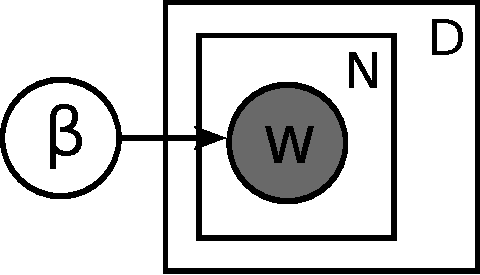
\includegraphics[width=0.2\textwidth]{chapter_introductory_material/figs/bagofwords_gm.pdf} & 
      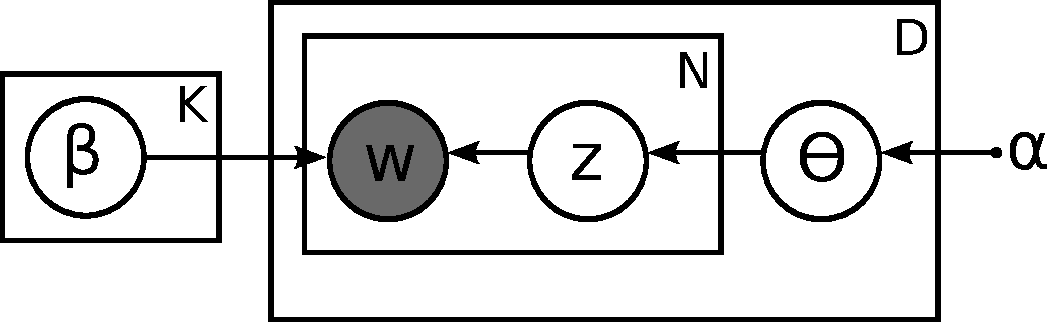
\includegraphics[width=0.4667\textwidth]{chapter_introductory_material/figs/lda_gm.pdf} \\
      Unigram language model & Latent Dirichlet allocation \\
    \end{tabular}
  \end{center}
  \caption{Left: graphical model for a unigram language model.
    Documents $1, \ldots, D$ are treated as \emph{bags of words}, or
    collections of words $w_n$.  Right: graphical model for Latent
    Dirichlet Allocation.  Circles are random variables, arrows
    connote dependency, and plates represent replication.  The circles
    represent observed random variables (words in this case).}
  \label{fig:bagofwords_lda_gm}
\end{figure}

One of the most useful assumptions we can make about a probability
distribution is conditional independence between groups of random
variables.  Given random variables $Z_1, Z_2$, and $Z_3$, we say that
$Z_1$ is conditionally independent of $Z_2$ given $Z_3$ if $p(Z_1, Z_2
| Z_3) = p(Z_1 | Z_3) p(Z_2 | Z_3)$ \citep{bishop:2006}.  Conditional
independence statements about distributions can often be inferred from
these distributions' factorizations \citep{bishop:2006} and become
important when one implements a probabilistic model or makes
predictions with one.

Before proceeding further, it is worth noting the benefits in using
latent-variable models.  Several of the most compelling motivations are:

  \begin{enumerate}
    \item Flexibility. These models can describe, summarize, and explain
    a wide variety of phenomena in the physical and social sciences.
  \item Embeddability and interpretability.  Any quantifiable metric
    in the dataset can be encoded as a random variable in a
    probabilistic model.  Relationships
    found within datasets can be likewise encoded
    explicity. \label{lvm:matching}
    \item Modularity. Parts of these models can be re-used across
      different models.  This leads to efficient transfer of resources
      and common paradigms.
    \item Existing toolbox of statistical tools. There is a large and
      growing body of literature around how to fit these models, and
      there are many widely supported packages for fitting these
      models.  Practitioners no longer need to be experts in
      statistics to correctly apply many of these tools.
  \end{enumerate}

  The risk with applying latent-variable models is that the
  credibility and careful deliberation we often associate with
  statistics lends credence to results of fitting a model.  This may
  lead researchers to be overconfident in the conclusions they draw
  from their models, particularly when the model is incorrectly
  interpreted, when the data is poorly fit by the model, or when the
  model is poorly defined.  Both of these can easily happen when
  Step~\ref{lvm:matching} above is carried out carelessly.

\subsection{Text as a medium for social science analysis}
  \label{sec:text_intro}
  We first illustrate these ideas in an application of text modeling.
  As noted in the last chapter, text data is as easy to work with as
  it is ubiquitous. Importantly, researchers and other practitioners
  are becoming more proficient with tools for text analysis.
  \cite{grimmer:submitted} provides an excellent overview of methods
  for analyzing text for social scientists; we will summarize several
  like methods here.

% \subsection{Latent-variable models of text}
  
  Text data is extremly high-dimensional.  A large collection of
  documents represented by a sequence $\bm w_n$ of words would be
  unweildly for even a human to describe.  A number of tools have been
  developed over the past several decades to simply find the
  \emph{gist} of documents, making it possible to describe collections
  succinctly and efficiently.

  In this work we will use the simplifying assumption that each text
  document is described by a vector $\bm w_d \in \mathcal{R}^V$ of
  word counts.  This assumption, known as the \emph{bag of words}
  assumption, removes most of the information in a document (here we
  use ``information'' in a very loose sense).  At the same time, this
  assumption still allows us to capture the ``gist'' of a document
  very well. One of the simplest bag-of-words models is the unigram
  model. In the unigram model, every word is assumed to come from the
  some multinomial distribution $\beta$ over the vocabulary:
  \[
    p(w_{11}, \ldots, w_{ND}) = p(\beta) \prod_D \prod_{N_d} p(w_{nd} |
  \beta). \]
  We illustrate this model graphically in
  \myfig{bagofwords_lda_gm} (A).  The bag-of-words assumption in
  particular is illustrated by the model's agnostic treatment of the
  order between words: these words are fully exchangeable within each
  document.

\subsubsection{Latent Dirichlet Allocation}
We will capture the gist of documents using the topic model Latent
Dirichlet Allocation \citep{blei:2003}.  Latent Dirichlet allocation
(LDA) posits a set of $K$ \emph{topics} $\beta_1, \ldots, \beta_K$ to
formalize what we mean by the \emph{gist} of a document.  LDA
describes each document $d$ as a mixture $\bm \theta_d$ of $K$ topics, where $\sum_K \theta_{dk} = 1$ and $\theta_{dk} > 0
\forall d,k$.

Formally, we represent this using a \emph{generative process} of the
collection of documents.  The generative process can be interpreted as
a recipe for creating the observations -- documents, in our case:
\begin{enumerate}
  \item Draw topics $\beta_1, \ldots, \beta_K \sim \mbox{Dir}(\eta)$.
    \item For document $d=1, \ldots, D$:
    \begin{enumerate}
    \item Draw topic mixture $\theta_d \sim \mbox{Dir}(\alpha, \ldots, \alpha)$.
    \item For term $n=1, \ldots, N$:
      \begin{enumerate}
      \item Draw topic indicator $z_n \sim \mbox{Mult}(\theta_d)$.
      \item Draw word $w_n \sim \mbox{Mult}(\beta_{z_n})$.
      \end{enumerate}
    \end{enumerate}
\end{enumerate}
The parameter $\alpha > 0$ above is a Dirichlet prior (it is often set by
topic model researchers to $1/K$).  The distribtion $\mbox{Dir}(\alpha_1, \ldots, \alpha_M)$ refers to the Dirichlet distribution.  Its density is given by
\begin{align}
  p(x_1, \ldots, x_M | \alpha_1, \ldots, \alpha_M) =
  \frac{\large \Gamma \left( \sum_{i=1}^M \alpha_i \right)}
       {\prod_{i=1}^M \large \Gamma(\alpha_i)}
       \prod_{i=1}^M x_i^{\alpha_i - 1}
\end{align}

We illustrate this model graphically in \myfig{bagofwords_lda_gm}.  Given the graphical model, we can immediately write the joint distribution of a collection of $D$ documents as
\begin{align}
  p(\beta_k, \theta, \bm Z, \bm W | \alpha) = 
  \prod_K p(\beta_k)
  \prod_D p(\theta_d) \prod_N p(z_n | \theta_d) p(w_n | z_n, \beta_{z_n}) d\beta d\theta dz,
\end{align}
where $p(\beta_k)$ and $p(\theta_d)$ are understood to be conditioned
on $\eta$ and $\alpha$ respectively (we treat $\alpha, \eta$ as
hyperparameters and omit them so they're not confused with random
variables).

In the vast majority of cases, the practitioner observes the words of
a set of documents and seeks to learn the topics that describe these
documents.

Before describing how to fit such a model, we point the reader to the
four example topics from LDA in \mytab{example_lda_topics}.  Note that
some of these ``words'' are instead phrases.  This can be done by
creating a vocabulary of phrases instead of words and describing
documents as a mixture of phrases.  We will describe how to select a
vocabulary of these phrases in
\myapp{issue_corpus_preparation}.
\begin{table}
  \caption{Example topics from Latent Dirichlet Allocation fit to sentences from the the textbook \emph{Biology} by Campbell and Reece.  This is a small subset of the 1000 topics. (These topics were provided by Ricky Wong.)}
  \center  \begin{tabular}{|c|c|c|c|}
% tissue bone collagen connective connective_tissue cartilage bones fibers 
% population growth rate age rates population growth populations life mortality
% dinosaurs dinosaur birds pterosaurs cretaceous bird long flight feet 
% forest diversity plant ectomycorrhizal fungi fungal treatment emf effects 
    \hline
    virus & forest & population & dinosaurs \\
    viruses & diversity & growth & dinosaur \\
    viral & plant & rate & birds \\
    host & ectomycorrhizal & age & pterosaurs \\
    phage & fungi & rates & cretaceous \\
    rna & fungal & population growth & bird \\
    genome & treatment & populations & long \\
    infection & emf & life & flight \\
    cell & effects & mortality & feed \\
    \hline
  \end{tabular}
  \label{fig:example_lda_topics}
\end{table}

\subsubsection{Inference}
Of course, we only observe the words $\bm Z$ in a collection of
documents, and we are interested in estimating what the topics $\beta$
and topic mixtures $\theta$ are.  We will generally accomplish this
with posterior inference, in which we aim to estimate the posterior
distribution
\begin{align}
  p(\beta, \theta, \bm Z | \bm W) = \frac{p(W | \beta, \theta, \bm Z) p(\beta, \theta, \bm Z)}{p(\bm W)}.
\end{align}

This conditional distribution is impossible to compute because of the
intractable normalizing constant
\begin{align} 
  p(\bm W) = & \prod_K \int_{\beta_k} p(\beta_k)
  \prod_D \int_{\theta_d} p(\theta_d | \alpha) \prod_N \sum_{n=1}^N p(z_n | \theta_d) p(w_n | z_n, \beta_{z_n}) d\beta d\theta dz.
\end{align}
\mysec{variational_inference} provides details on how to get around
this by approximating the posterior above.

We will use topic models like LDA for several purposes in later
sections.

%\subsubsection{Unigram models}
%  One of the simplest bag-of-word language models is a unigram model

%\subsubsection{Regression}
% One of these applications is prediction. In the simplest of these   In text regressionWe will see in later sections that topic models can be used for
% prediction by using Text regression is a

\subsection{Matrix factorization, latent space models, and
  multidimensional scaling}

Two of the most common primitives in latent-variable models are matrix
factorization \citep{salakhutdinov:2008a} and multidimensional scaling,
which describe relationships between pairs of items, or dyads. We
first discuss a specific application of matrix factorization called
item response theory (IRT), which has been used for decades in
political science
\citep{clinton:2004,martin:2002,poole:1991,enelow:1984,albert:1992}.

In IRT, we have two types of objects, and we would like to make
predictions about pairs of them.  Each of these objects -- suppose
that they are lawmakers and bills, to be concrete -- is represented by
real-valued random variables: lawmaker $u \in \{ u=1, \ldots, U \}$
has a latent value $X_u \in \mathbb{R}$, and each bill $d \in \{ 1,
\ldots, D \}$ has two latent values $A_d,B_d \in \mathbb{R}$.  We make
predictions about pairs of them by introducting the likelihood
function $p(V_{ud} | X_u, A_d, B_d) = \sigma( x_u a_d + b_d )$, where
$\sigma(s) = \frac{\exp(s)}{ 1 + \exp(s) }$.

More formally, we can say that the matrix $\{V\}_{ud}$ of boolean outcomes (for example, votes) is represented with the matrix product
\begin{align}
  \hat \sigma \left( \left[ \begin{array}{cc}
    x_1 & 1 \\
    \vdots & \vdots \\
    x_U & 1 \\
  \end{array}
  \right]
  \left[
    \begin{array}{ccc}
      a_1 & \cdots & a_D \\
      b_1 & \cdots & b_D \\
    \end{array}
    \right]
  \right),
\end{align}
where the matrix operator $\hat \sigma(\cdot)$ produces a matrix in
which the scalar logistic function $\sigma(s) = \frac{\exp(s)}{1 +
  \exp(s)}$ is applied to each element of its argument.

\begin{figure}
  \begin{center}
  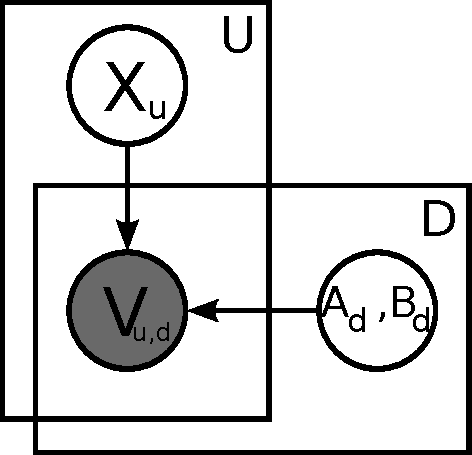
\includegraphics[width=0.3\textwidth]{chapter_introductory_material/figs/irt_gm.pdf}
  \end{center}
  \caption{Probabilistic matrix factorization.  We observe
    interactions $V_{ud}$ between users represented by $X_u$ and items
    represented by $A_d, B_d$.}
  \label{fig:irt_gm}
\end{figure}

A wide variety of researchers have used formulations like this for
applications such as recommendation and representing the votes of
lawmakers
\citep{wang:2011,salakhutdinov:2008a,poole:1985,poole:1991,clinton:2004}. In
later chapters, we will use it for models of legislative voting.

Sometimes these pairs of items that interact in dyads are of the same
``type'', and we wish to model them in the same latent space.  Instead
of bills and lawmakers interacting, for example, we will also consider
pairs of countries that interact, and we wish for these countries to
be represented in the same latent, interpretable space.  In this case,
we will still model each country with a latent position vector $\bm
x_u$, and we will model their interaction as above, with
\[
  p(v | \bm x_i, \bm x_j) = \sigma(\bm x_i^T \bm x_j),
\]
for a suitable distribuiton $\sigma$.  We will also frame their
relationship using their Euclidean distance
in this latent space:
\[
  p(v | \bm x_i, \bm x_j) = \sigma(\bm \beta w_{ij} - || \bm x_i - \bm x_j ||_2),
\]
where $w_{ij}$ are observed covariates about the dyad and $\bm \beta$
is hidden along with $\bm x$ \citep{hoff:2002}. Both of these
formulations will allow us to develop a model of foreign relations in
\mychap{foreign_relations}.

% Recent 
%   - relevant sources
%   - mathematical foundation
%   - examples
%   - hinge loss
%   - inference (stochastic)

\subsection{Hidden Markov Models and Kalman Filters}
We now turn briefly to abstractions for time-series data. One of the
simplest assumptions about a time-series colleciton is that we have a
sequence of observations $Y_1, \ldots, Y_T$ observed at times $t=1,
\ldots, t=T$.  In a \emph{hidden Markov model} (HMM).  We assume that
these observations can be explained by a hidden set of states $X_1,
\ldots, X_T$, which are temporally linked.  The model factorizes as
\begin{align}
  p(Y_1, \ldots, Y_T, X_1, \ldots, X_T) = p(X_1) p(Y_1 | X_1) \times \prod_{t=2, \ldots, T} p(X_t | X_{t-1}) p(Y_t | X_t)
\end{align}
(see \myfig{hmm_gm} for the graphical model).  Often the transition
distribution $p(X_t | X_{t-1})$ is independent of $t$ (the chain in
this case is called \emph{time-homogenous}).  A wide variety of
problems can be modeled accurately with a well-selected homogeneous
HMM.  Importantly, inference in these models is very efficient because
the set of conditional independencies yields a tree: inference can
usually be reduced to an application of a forward-backward algorithm,
especially when the conditional distribution of each variable given
its neighbor is conjugate (even when this is not the case, recent
methods provide approximate ways to infer an HMM (Paisley, Gerrish,
and Blei 2010).
\nocite{paisley:2010})
One of the most famous examples of a hidden Markov model is the Kalman
filter, which assumes linear (or quadratic) transitions between the
states $X$ and Gaussian noise: $p(Y_t | X_t) \propto \mathcal{N}(X_t,
\sigma^2)$ for some variance $\sigma^2$.
\begin{figure}
  \begin{center}
  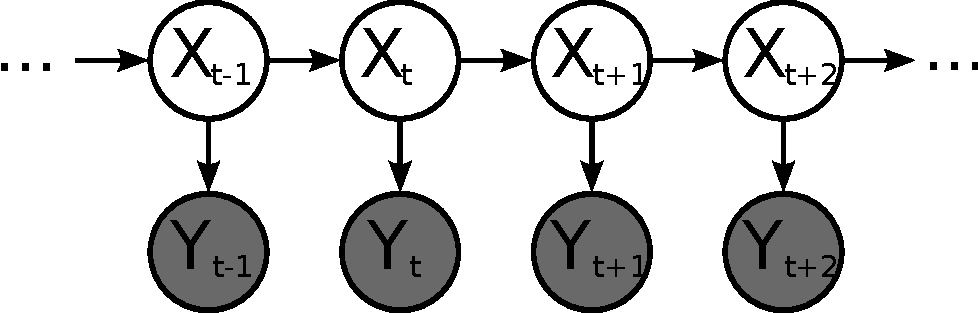
\includegraphics[width=0.6\textwidth]{chapter_introductory_material/figs/hmm_gm.pdf}
  \end{center}
  \caption{A hidden Markov model.  Observations $Y_1, \ldots, Y_T$ are observed at discrete times $t=1, \ldots, T$, and are conditionally independent given the hidden states $X_1, \ldots, X_T$.}
  \label{fig:hmm_gm}
\end{figure}

We will these time-series abstractions in modeling time-series
collections of documents.  In these collections, the assumption of a
hidden, evolving state will allow us to perform inference efficiently
while inferring a sequence of states which can be interpreted---for
example, we will use this to model themes which evolve over time in
Chapter 2 and to infer countries' positions about foreign policy
issues in Chapter 3.

We have discussed text and time-series assumptions, which are often
seen together in the context of natural language processing.  We will
not use time-series assumptions at the level of syntactic language
modeling.  While sequential modeling is useful for many NLP tasks, we
will not use them in this work, instead deferring to the bag-of-words
assumption described in \mysec{text_intro}.

% TODO(sgerrish): cite Kalman.

\section{Posterior inference and model evaluation}
One of the most fundamental problems in statistical machine learning
is that of estimating the values of latent random variables $X$ in a
statistical model, given observed random variables $Y$ (i.e., data).
In this thesis, we will frequently need to estimate the posterior distribution
$p(x | y) = \frac{p(x, y)}{p(y)}$.  In this section I outline
several common methods for estimating this posterior.

\subsection{MAP estimation}
One of the simplest estimates of the value of a random variable is the \emph{maximum-a-posteriori} (MAP) estimate.  The MAP estimate $\hat X$ is defined to be the most-likely value of the random variable:
\begin{align}
  \hat X = \arg \max_x p(X=x | Y) = \arg \max_x \frac{p(X=x | Y) p(Y)}{p(Y)} = \arg_x \max p(X=x, Y).
\end{align}

The MAP estimate can typically found by performing gradient or
coordinate ascent on $p(X, Y)$ with respect to $X$ (this is because
the normalizer $p(Y)$ is not a function of $X$).  Because MAP
estimates can be fast to estimate, they can shorten the development
loop described in \mysec{pipeline}. The MAP provides a point estimate
which is often a good summary of the posterior distribution.

\subsection{MCMC}

% Markov Chain Monte-Carlo (MCMC) methods provide a method for drawing
% samples $x_m$ from a posterior distribution $p(X | Y)$.

We briefly review the key components of Markov Chain Monte Carlo
(MCMC) estimation.  We will not go into detail about MCMC in this work
except to build up to (and draw a contrast with) variational methods,
which are introduced in the next section. Readers unfamiliar with MCMC
can refer to a standard text such as \cite{bishop:2006}.

% Markov Chain Monte-Carlo methods provide non-independent samples from
% a posterior.  These samples are unbiased, and, when the number of
% samples is large, they can be used to reliably estimate arbitrary
% statistics of a posterior distribution (such as marginal mean and
% variance).

MCMC methods are often used to inspect a posterior distribution $p(x |
y)$.  The input to an MCMC sampler is typically an unnormalized
probability density $\tilde p(x, y) \propto p(x | y)$ \footnote{For
  numerical and algebraic convenience, $\tilde p(x, y)$ is often
  specified by $\log \tilde p(x, y)$.}  Given $\tilde p(x, y)$, an
MCMC sampler produces a collection of samples from $p(x | y)$.  These
samples are often used to summarize statistics such as marginal means
and variances of $p(x | y)$.  They are unbiased and, given enough
time, will accurately represent $p(x | y)$.

MCMC methods are used widely, but they have limitations.
One of these limitations is runtime: while one may need $N$ \emph{iid}
samples from a distribution $p(x | y)$ to estimate its mean and
variance, he typically needs many more MCMC samples to estimate these
statistics.  A poorly-chosen proposal distribution can affect runtime,
as a Markov chain needs more samples to converge. MCMC algorithms can
also suffer from memory bottlenecks, as samples are stored and
convergence is measured.

Even when memory is not a bottleneck, the practitioner is often
interested in only the marginals of the posterior (as with most
mixture-of-Gaussian applications); a large number of discarded samples
indicates that there is an inefficiency in the inference pipeline.

\subsection{Variational inference}
\label{sec:variational_inference}

Variational methods address some of the shortcomings of MCMC by
providing a fast, deterministic alternative to MCMC
\citep{jordan:2003,jordan:1999}. These algorithms have been
successfully applied to many kinds of topic models, where corpus size
and vocabulary dimension are large.  We review the key ideas of
variational inference here for use in later chapters.

Variational methods posit a simplified\footnote{Simplified compared to
  the true posterior.} family of probability distributions, indexed by
variational parameters $\theta$, and select the member $q_\theta$ of
this family that is closest in KL-divergence to the true posterior
$p(x | y)$:
\begin{align}
  \arg \min_{\theta} \mbox{KL}(q_\theta || p) = \arg \min_{\theta} \int_x q_\theta(x) \log \frac{q_\theta(x)}{p(x | y)} dx.
  \label{eq:variational_objective}
\end{align}
Finding the optimal variational distribution $q_\theta$ is equivalent
to optimizing an ``evidence lower bound'' (ELBO) ($\mathcal{L}_\theta$) on
the data likelihood
\begin{eqnarray}
  \log p(y) \ge & \expectq{\log p(x, y) - \log q_\theta(x)} \\
  = & \expectq{\log p(x, y)} - H(q_\theta(x)) \\
  =:&  \mathcal{L}_\theta,
  \label{eq:traditional_variational_objective}
\end{eqnarray}
where $H(q_\theta(x))$ is the entropy of that distribution and the
slack of the bound is equal to the KL divergence from
Equation~\ref{eq:variational_objective}.

The family is chosen by the practitioner to make the resulting
algorithm tractable and to capture the parameters of interest. A
common assumption is that the posterior is fully-factorized into
simple marginal distributions; such an assumption is known as
\emph{naive mean-field variational inference}. Though simpler, the
fitted variational distributions are found to be good proxies for the
true posterior~\citep{jordan:1999,gerrish:2011}.

\begin{figure}
  \center
  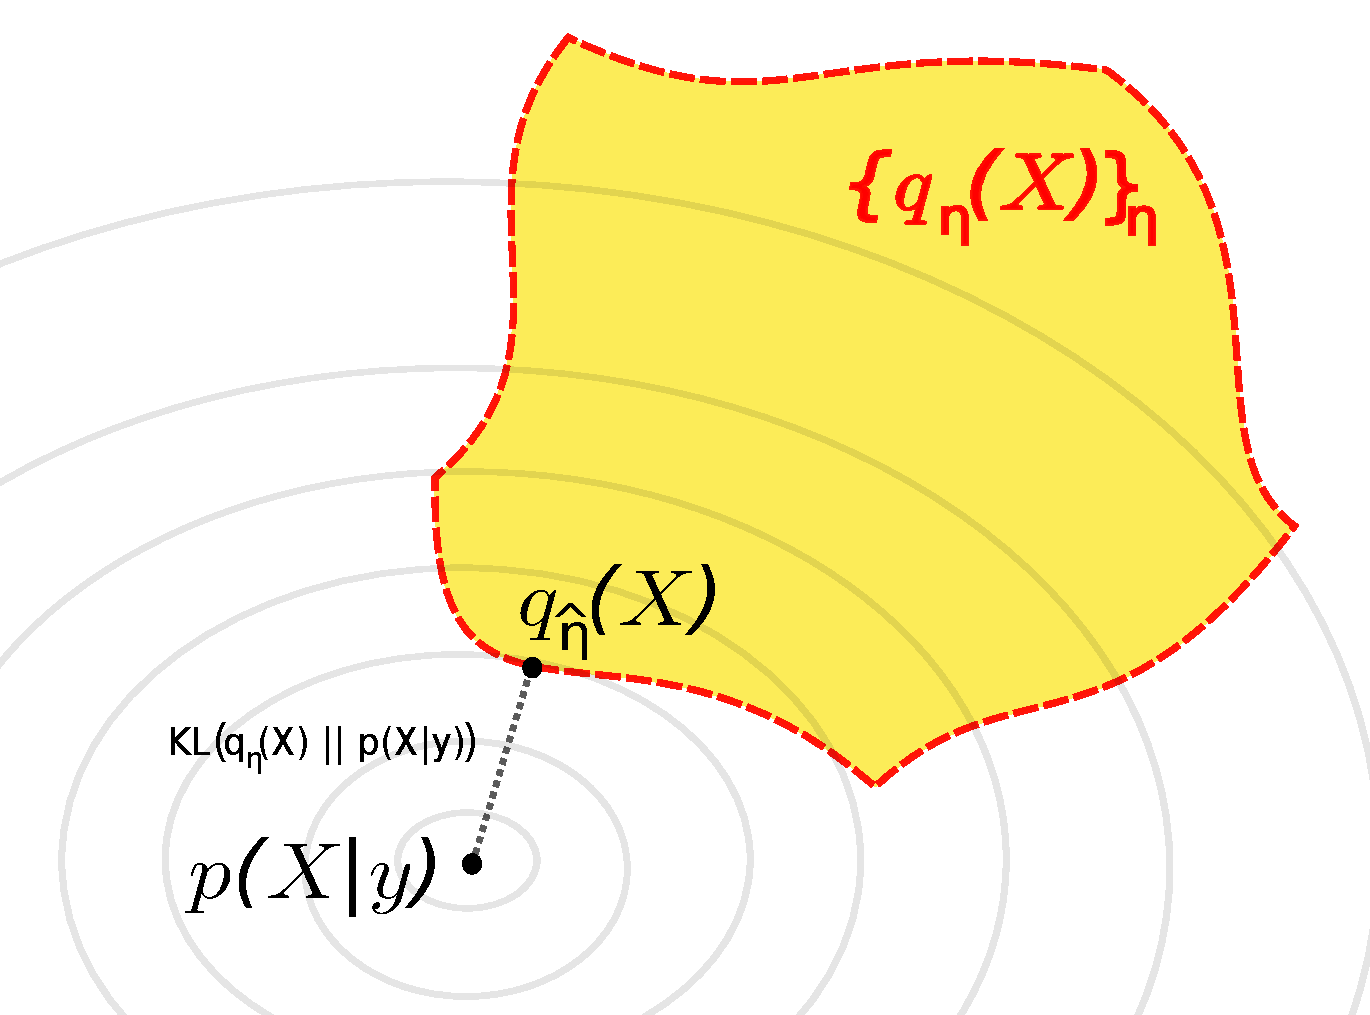
\includegraphics[width=0.6\textwidth]{chapter_introductory_material/figs/variational_family.pdf}
  \label{fig:variational_inference}
  \caption{Illustration of variational inference.  Practitioners
    define a variational family (shaded yellow region) and find the
    member of that family $q_{\hat \eta}(x)$ which is closest (by KL
    divergence) to the true posterior.}
\end{figure}
For example, a multivariate posterior $p(x | Y), x \in \mathcal{R}^D$
might be represented by the product $q(x_{1:D}) = \prod_D
\mathcal{N}(x_d | \mu_d, \sigma_d^2)$ of $D$ Gaussian distributions,
and a multinomial posterior might be represented by a Dirichlet
distribution \citep{bishop:2006}.  In the case of Latent Dirichlet
Allocation, for example, \cite{blei:2003} assume that the indicators
$z_n$ can be described by a fully-factorized product of multinomial
distributions, and they assume that the posterior distribution of
topics $\beta$ and mixture proportions $\theta$ can be represented by
a fully-factorized product of Dirichlet distributions.

Once a family is selected, the bound in
Equation~\ref{eq:traditional_variational_objective} is evaluated
symbolically, as a practitioner fully expands $\expectq{ \log p(x, y)
  - \log q_\theta(x)}$ and (usually) its gradient. As we will show in
subsequent chapters, this bound may itself be bounded or approximated
with a Taylor approximation such as the delta method
\citep{bickel:2007,braun:2007}. These simplifying assumptions -- an
approximate, fully factorized posterior with further simplifying
bounds -- make it possible to express the lower bound in terms of the
variational parameters $\theta$.  The practitioner then uses these
bounds and gradients in a coordinate or
gradient ascent algorithm.

The role of variational inference in statistical machine learning will
become more clear as we develop several algorithms using these methods
over the next few chapters.  We will also introduce an alternative
method for performing variational inference in
Appendix~\ref{chapter:stochastic_variational_optimization}.  This
alternative method removes the onus of deriving new variational update
equations, making it easy for the practitioner to perform rapid model
development on a range of models.

% \subsection{Stochastic optimization}
%   - examples

% \subsection{Posterior Predictive Checks}
%   - examples
\subsection{Model evaluation}
After a model has been fit with an approach such as variational
inference, it is important to evaluate the model (see again the data
analysis pipeline in \mysec{data_analysis_pipeline}).  In general,
different practitioners will have different goals in modeling data, so
they will have different goals in model evaluation.  However, several
standard approaches exist.

\subsubsection{Likelihood of training data $Y_1, \ldots,
  Y_{N_{\mbox{\small obs}}}$}
We first describe one of the simplest metrics of how well a model is fit:
its ability to model training data $Y_{\mbox{\small obs},1},$
$\ldots,$ $Y_{\mbox{\small obs},N_{\mbox{\tiny obs}}}$.  Like before,
one of the most frequently used metrics for this is the training
log-likelihood $\log p(Y_{\mbox{\small obs},1}, \ldots,
Y_{\mbox{\small obs},N_{\mbox{\tiny obs}}})$ of these
observations. When these observations are conditionally independent
given the observed data (nearly always the case), the log-likelihood
can be written $\sum_{n=1}^{N_{\mbox{\tiny obs}}} \log
p(Y_{\mbox{\small obs},n})$.  The downfall of this metric is of course
that it does not measure whether a model is overfit.  However, it is
the objective function used when an MAP or MLE estimate is
fit.  In addition, it can be used to measure the flexibility of a model.

% \subsubsection{Predictive accuracy}
% When a model is created for the purpose of making predictions, heldout
% log-likelihood is often not an appropriate measure of that model's
% performance.  To be concreate, consider a model developed to predict
% the maximum

% \subsubsection{Relationship with external observations}
% Sometimes a model A final metric that we will consider is a model's
% relationship to outside data -- data which was not directly
% incorporated into the model.

% In a model we will develop later, we are operating in a
% vacuum: This can be useful when, for example, the model

\subsubsection{Likelihood of heldout observations $Y_1, \ldots,
  Y_{N_{\mbox{\small heldout}}}$}
One of the most common metrics of a model is its ability to model
unseen, heldout observations $Y_{\mbox{\small hdt},1},$ $\ldots,$
$Y_{\mbox{\small hdt},N_{\mbox{\tiny hdt}}}$ given a set of ``training''
  observations $Y_{\mbox{\small h},1},$ $\ldots,$ $Y_{\mbox{\small
      h},N_{\mbox{\tiny obs}}}$ One of the most frequently used metrics
    for this is the log-likelihood
\begin{align*}
  \log
  p(Y_{\mbox{\small hdt},1}, \ldots, Y_{\mbox{\small hdt},N_{\mbox{\tiny hdt}}}
  | Y_{\mbox{\small obs},1}, \ldots, Y_{\mbox{\small obs}, N_{\mbox{\tiny obs}}})
\end{align*}
of these observations. When these observations are conditionally
independent given the observed data (nearly always the case), the
log-likelihood can be written $\sum_{n=1}^{N_{\mbox{\tiny hdt}}} \log
  p(Y_{\mbox{\small hdt},n} | Y_{\mbox{obs},1}, \ldots, Y_{\mbox{\small obs},N_{\mbox{obs}}})$.

When training data is scarce, practitioners often use leave-one-out
cross-validation.  Cross-validation requires that the training data be
partitioned into $K$ equal-size parts $P_1, \ldots, P_K$, fit $K$
times on each of the $K - 1$ subsets which omit exactly one of the
partitions, and evaluated on the omitted partition.  Such a model has
the benefit that all of the data is used for training and evaluation.

\subsubsection{Relationship with external data}
In this thesis we will use external data sources to validate the
results of our model.  External data sources are useful because they
can confirm a model's assumptions or 

\section{Using these tools to understand influence and decisionmaking}

The ideas outlined in this chapter cover only the tip of the iceberg
of the set of tools used by statistical machine learning researchers
(and this is only a subset of all machine learning researchers).
However, they will serve as important building blocks for future
chapters.  In the next chapter we will use some of these ideas as we
return to the original questions that motivated this thesis: how can
we understand patterns of behavior in society using text?  How do
documents interact with one another, and how can we use them to tell
us how people interact with the world?

We will use the tools discussed in the preceeding sections to shed
light on these questions, and we will do this with exactly the
data-analysis recipe that we outlined in
\mysec{data_analysis_pipeline}.  This recipe involves defining a question,
describing a model to answer that question using data, fitting that
model, and drawing inferences from the model.
 
In the next chapter we will return to a fundamental challenge in
managing the huge volumes of text now inundating researchers and
companies: how to find the most important and influential documents in
a collection.  As we will show in the next chapter, a latent-variable
treatment of this question will allow us to make our assumptions
explicit.  This in turn will in turn make the subsequent analysis
straightforward.
